%==============================================================================
%  Few-Shot Open-Set Keyword Spotting at Vocabulary Scale
%  Single-file LaTeX source, ready to paste into Overleaf.
%
%  Recommended compiler: pdfLaTeX (Overleaf default).
%  All tables/figures are self-contained (no external data files required).
%==============================================================================
\documentclass[10pt,twocolumn]{article}

%------------------------------ packages --------------------------------------
\usepackage[utf8]{inputenc}
\usepackage[T1]{fontenc}
\usepackage[english]{babel}
\usepackage{lmodern}
\usepackage{microtype}
\usepackage[a4paper,margin=2cm]{geometry}

\usepackage{amsmath,amssymb,amsfonts}
\usepackage{graphicx}
\usepackage{booktabs}
\usepackage{multirow}
\usepackage{array}
\usepackage[table]{xcolor}
\usepackage{enumitem}
\usepackage{caption}
\usepackage{subcaption}
\usepackage{algorithm}
\usepackage{algpseudocode}
\usepackage{tikz}
\usepackage{pgfplots}
\pgfplotsset{compat=1.18}
\usetikzlibrary{arrows.meta,positioning,fit,backgrounds,calc}
\usepackage[hidelinks,colorlinks=true,linkcolor=blue!55!black,citecolor=blue!55!black,urlcolor=blue!55!black]{hyperref}
\usepackage{cleveref}

%------------------------------ helpers ---------------------------------------
\newcommand{\best}[1]{\textbf{#1}}
\newcommand{\pms}[2]{$#1\,{\scriptstyle\pm\,#2}$}     % mean +- std
\newcommand{\acc}{\text{ACC}}
\newcommand{\far}{\text{FAR}}
\newcommand{\frr}{\text{FRR}}
\newcommand{\eer}{\text{EER}}
\newcommand{\auc}{\text{AUC}}
\newcommand{\R}{\mathbb{R}}
\newcommand{\norm}[1]{\lVert #1\rVert}
\newcommand{\code}[1]{\texttt{\small #1}}

\captionsetup{font=small,labelfont=bf}

%==============================================================================
\begin{document}

\twocolumn[
\begin{@twocolumnfalse}
\begin{center}
{\LARGE\bfseries Few-Shot Open-Set Keyword Spotting at Vocabulary Scale:\\[2pt]
A Metric-Learning Study of Encoders, Losses, and Open-Set Rejection\par}
\vspace{8pt}
{\large Author Name\textsuperscript{1} \quad Advisor Name\textsuperscript{1}\par}
\vspace{4pt}
{\itshape \textsuperscript{1}Department of \dots, University \dots\par}
\vspace{4pt}
{\small \href{mailto:author@example.com}{author@example.com}\par}
\vspace{12pt}

\begin{minipage}{0.92\textwidth}
\small
\textbf{Abstract.}
We study \emph{few-shot open-set keyword spotting} (KWS): a single embedding
encoder is trained once on a large word vocabulary and is then deployed to
recognize an \emph{arbitrary} user-defined keyword set from only a handful of
enrollment examples, while rejecting out-of-vocabulary speech and silence. We
build a fully reproducible pipeline around two compact encoders --- a
depthwise-separable CNN (DSCNN-L, $\approx$0.41\,M parameters) and a temporal-attention
edge model (EdgeSpot-Full~$\tau{=}4$, $\approx$0.13\,M parameters) --- combined with three
feature front-ends (MFCC, log-mel, and a trainable per-channel PCEN) and four
metric-learning objectives (Triplet, Sub-center ArcFace (SCAF), Generalized
End-to-End (GE2E), and a cosine knowledge-distillation (KD) objective from a
frozen Wav2Vec\,2.0 teacher). All systems are trained on Multilingual Spoken
Words Corpus (MSWC) English and evaluated cross-corpus on Google Speech Commands
v2 (GSC) under a strict \emph{EdgeSpot-exact} 10-shot open-set protocol with 100
randomized runs. Through a 16-configuration factorial screen we show that
(i) the trainable PCEN front-end is the single most reliable improvement
(up to $+9.2$ accuracy points at $1\%$ false-accept rate for the edge encoder);
(ii) the centroid-based GE2E objective dominates classification-style losses for
open-set generalization; and (iii) crucially, the classification objective SCAF
\emph{collapses} when the training vocabulary grows to $37{,}387$ classes
unless its loss weight is reduced by four orders of magnitude. We further
characterize how accuracy \emph{saturates} near two million training clips and
show that the cosine-KD objective reaches GE2E-level accuracy with roughly half
the data. The best overall configuration (DSCNN-L\,+\,PCEN\,+\,GE2E) attains
\best{$86.36\%$} open-set accuracy at $1\%$ false-accept rate and \best{$95.21$}
AUC on GSC test, while the best compact model (EdgeSpot-Full\,+\,PCEN\,+\,GE2E)
reaches $82.87\%$ at one third of the parameters. We release the complete code,
training/evaluation protocols, and an offline web demonstrator.

\vspace{6pt}
\noindent\textbf{Keywords:} keyword spotting, few-shot learning, open-set
recognition, metric learning, prototypical networks, GE2E, PCEN, knowledge
distillation, edge AI.
\end{minipage}
\end{center}
\vspace{14pt}
\end{@twocolumnfalse}
]

%==============================================================================
\section{Introduction}\label{sec:intro}

Keyword spotting (KWS) --- the task of detecting a small set of spoken commands
in a continuous audio stream --- is the always-on entry point of nearly every
modern voice interface. Classical KWS systems are trained as \emph{closed-set}
classifiers over a \emph{fixed} vocabulary (e.g., the ten Google Speech Commands
words). This design has two structural limitations. First, the keyword set is
frozen at training time: supporting a new wake word or command requires
collecting data and retraining the model. Second, a softmax classifier is, by
construction, \emph{not} open-set: every input is forced into one of the known
classes, so unseen words and background noise are silently misclassified as
commands, producing false activations.

This work targets the more realistic and more difficult
\textbf{few-shot open-set} formulation. We train a single \emph{embedding
encoder} on a very large and diverse word vocabulary, and at deployment time the
end user defines an \emph{arbitrary} keyword set by providing only a few
($k$) enrollment utterances per word. Each keyword is represented by a
\emph{prototype} (the mean embedding of its enrollment shots); recognition is
performed by nearest-prototype matching in embedding space, and an explicit
open-set decision rejects anything that is too far from all prototypes. Because
the encoder is never retrained for a particular keyword, the same model serves
unlimited downstream vocabularies; because rejection is distance-based, the
system can abstain on out-of-vocabulary speech and silence.

The central scientific question we pursue is \emph{what makes such an encoder
generalize}, and in particular how the design choices interact with the
\emph{scale} of the training vocabulary. We perform a controlled factorial study
over three axes --- feature front-end, encoder backbone, and metric-learning
objective --- and we deliberately push the training vocabulary from a 31-word
``micro-set'' up to the full $37{,}387$-word MSWC English corpus. This scaling
exposes a phenomenon that is invisible at small scale: a classification-style
angular-margin loss that is competitive on a few hundred classes
\emph{catastrophically collapses} on tens of thousands of classes.

\paragraph{Contributions.} Our main contributions are:
\begin{enumerate}[leftmargin=1.4em,itemsep=2pt]
\item A reproducible, dependency-light few-shot open-set KWS framework with two
compact encoders, three feature front-ends, four metric objectives, and four
open-set rejection heads (nearest-class-mean / OpenMax / energy / calibrated),
all sharing a common prototype interface (\Cref{sec:system,sec:openset}).
\item A 16-configuration factorial screen on full-vocabulary MSWC that isolates
the contribution of each axis with paired deltas; PCEN and GE2E emerge as the
two robust wins (\Cref{sec:matrix}).
\item A scale analysis showing (a) accuracy saturation near $\sim$2\,M training
clips and (b) the failure mode of Sub-center ArcFace at $37$k classes, with a
gradient-magnitude explanation and a practical fix (\Cref{sec:scale}).
\item A knowledge-distillation study showing that a cosine objective against a
frozen Wav2Vec\,2.0 teacher matches GE2E accuracy with roughly half the training
data (\Cref{sec:kd}).
\item A complete cross-corpus evaluation under a strict EdgeSpot-exact 10-shot
protocol (100 runs), together with a CPU streaming pipeline (Silero VAD +
smoothing state machine) and an offline web demonstrator (\Cref{sec:system-impl}).
\end{enumerate}

%==============================================================================
\section{Related Work}\label{sec:related}

\paragraph{Small-footprint KWS.}
Depthwise-separable convolutions popularized by DS-CNN~\cite{zhang2017hello}
remain a strong accuracy/size trade-off baseline for on-device KWS, later refined
by broadcasted-residual networks (BC-ResNet)~\cite{kim2021bcresnet}. Our DSCNN-L
encoder follows the DS-CNN size-table design, and our EdgeSpot encoders combine
fused/broadcasted temporal blocks with a single-head temporal self-attention
stage in the spirit of attention-augmented edge KWS.

\paragraph{Few-shot and metric-learning KWS.}
Treating KWS as metric learning enables flexible vocabularies. Prototypical
networks~\cite{snell2017prototypical} and triplet
embeddings~\cite{schroff2015facenet} provide the classic few-shot machinery;
GE2E~\cite{wan2018ge2e} was introduced for speaker verification and naturally
mirrors the enroll-then-classify deployment of few-shot KWS. We adopt GE2E as a
\emph{centroid} objective and compare it head-to-head with triplet and
classification objectives.

\paragraph{Angular-margin classification.}
ArcFace~\cite{deng2019arcface} and its sub-center
variant~\cite{deng2020subcenter} produce highly discriminative embeddings for
face recognition with thousands of identities. We test whether the same
machinery transfers to word embeddings at $10^4$-class scale and report a
negative result with a concrete remedy.

\paragraph{Open-set recognition.}
OpenMax~\cite{bendale2016openmax} rejects unknowns by Weibull tail modeling of
activations, and energy scores~\cite{liu2020energy} provide a calibration-free
alternative. We adapt both to operate on prototype distances and compare them to
a simple nearest-class-mean (NCM) distance threshold.

\paragraph{Front-ends and self-supervision.}
PCEN~\cite{wang2017trainable} is a trainable, per-channel adaptive gain/compression
front-end designed for robust far-field detection. Wav2Vec\,2.0~\cite{baevski2020wav2vec}
provides powerful self-supervised speech representations; we use a frozen
Wav2Vec\,2.0 as a distillation teacher rather than as the deployed model, keeping
the student tiny.

%==============================================================================
\section{Problem Formulation}\label{sec:problem}

Let $f_\theta:\R^{T\times F}\!\to\!\R^{d}$ be an encoder mapping a one-second
log-frequency representation to a unit-norm embedding,
$f_\theta(x)=\tilde z/\norm{\tilde z}_2$. At deployment the user supplies a
\emph{support set} of $k$ utterances per keyword $w\in\mathcal{K}$. The prototype
of $w$ is the mean support embedding
\begin{equation}
p_w \;=\; \frac{1}{k}\sum_{i=1}^{k} f_\theta\!\big(x^{(w)}_i\big).
\label{eq:proto}
\end{equation}
For a query $x$ we compute the nearest prototype and its distance,
\begin{equation}
\hat w(x)=\arg\min_{w\in\mathcal{K}} d\!\big(f_\theta(x),p_w\big),\qquad
s(x)=-\!\min_{w}\, d\!\big(f_\theta(x),p_w\big),
\label{eq:score}
\end{equation}
with $d$ the Euclidean distance. The \emph{open-set decision} accepts $x$ as the
keyword $\hat w(x)$ iff the score exceeds an operating threshold $\tau$, and
otherwise emits \texttt{unknown}:
\begin{equation}
\text{decision}(x)=
\begin{cases}
\hat w(x), & s(x)\ge \tau,\\[2pt]
\texttt{unknown}, & s(x)<\tau .
\end{cases}
\label{eq:decision}
\end{equation}
The encoder $\theta$ is trained on a \emph{disjoint} corpus and vocabulary; at
test time $\mathcal{K}$ and the threshold $\tau$ are chosen \emph{without}
updating $\theta$. The two coupled goals are (i) high keyword accuracy on the
known set and (ii) high rejection of unknown words and silence --- exactly the
detection/false-alarm trade-off captured by the DET curve.

%==============================================================================
\section{System Architecture}\label{sec:system}

\Cref{fig:pipeline} summarizes the end-to-end pipeline. We now describe each
stage with the exact configuration used in our experiments.

\begin{figure*}[t]
\centering
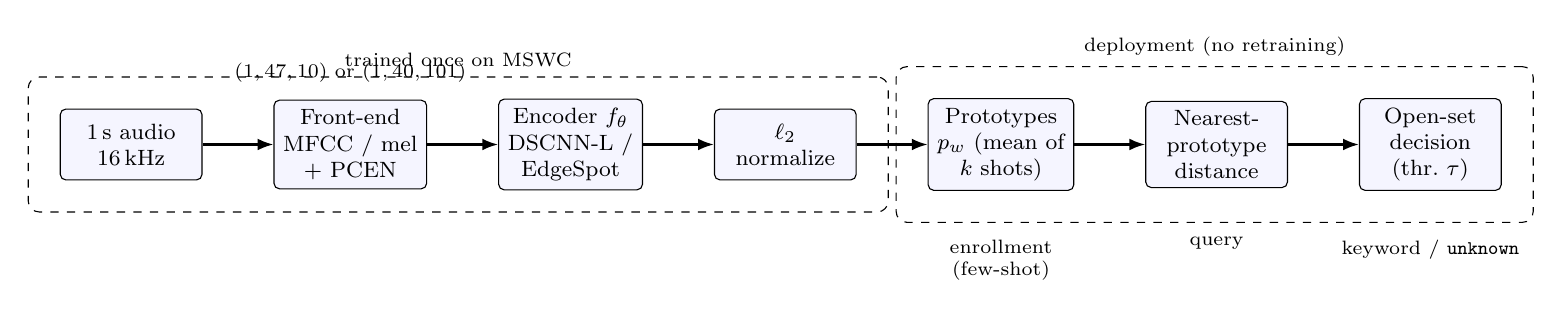
\begin{tikzpicture}[
  node distance=7mm and 9mm,
  box/.style={draw,rounded corners=2pt,align=center,minimum height=9mm,
              minimum width=18mm,font=\footnotesize,fill=blue!4},
  small/.style={font=\scriptsize,align=center},
  arr/.style={-{Latex[length=2mm]},thick}
]
\node[box] (wav) {1\,s audio\\16\,kHz};
\node[box,right=of wav] (feat) {Front-end\\MFCC / mel\\$+$ PCEN};
\node[box,right=of feat] (enc) {Encoder $f_\theta$\\DSCNN-L /\\EdgeSpot};
\node[box,right=of enc] (norm) {$\ell_2$\\normalize};
\node[box,right=of norm] (proto) {Prototypes\\$p_w$ (mean of\\$k$ shots)};
\node[box,right=of proto] (dist) {Nearest-\\prototype\\distance};
\node[box,right=of dist] (dec) {Open-set\\decision\\(thr.\ $\tau$)};

\draw[arr] (wav)--(feat);
\draw[arr] (feat)--(enc);
\draw[arr] (enc)--(norm);
\draw[arr] (norm)--(proto);
\draw[arr] (proto)--(dist);
\draw[arr] (dist)--(dec);

\node[small,above=1mm of feat] {$(1,47,10)$ or $(1,40,101)$};
\node[small,below=5mm of proto] {enrollment\\(few-shot)};
\node[small,below=5mm of dist] {query};
\node[small,below=5mm of dec] {keyword / \texttt{unknown}};

\begin{scope}[on background layer]
\node[draw,dashed,rounded corners,fit=(wav)(norm),inner sep=4mm,
      label={[font=\scriptsize]above:trained once on MSWC}] {};
\node[draw,dashed,rounded corners,fit=(proto)(dec),inner sep=4mm,
      label={[font=\scriptsize]above:deployment (no retraining)}] {};
\end{scope}
\end{tikzpicture}
\caption{End-to-end few-shot open-set KWS pipeline. The encoder is trained once
on MSWC; at deployment, user keywords are enrolled as prototypes and queries are
classified by nearest-prototype distance with an explicit open-set threshold.}
\label{fig:pipeline}
\end{figure*}

\subsection{Feature front-ends}\label{sec:features}

All audio is mono, $16$\,kHz, and trimmed/zero-padded to exactly one second
($16{,}000$ samples). We support two spectral parameterizations, summarized in
\Cref{tab:features}.

\paragraph{MFCC (DSCNN front-end).}
We compute $40$ Mel-frequency cepstral coefficients with a $1024$-point FFT,
$640$-sample ($40$\,ms) Hann window, $320$-sample ($20$\,ms) hop, and
\code{center=False}; the Mel filterbank uses Slaney scale and Slaney area
normalization, and the log is taken as $10\log_{10}(\cdot)$ followed by an
orthonormal DCT-II. We retain \emph{only the first $10$ coefficients} and
transpose to a tensor of shape $(1,47,10)=(\text{channel},T_{\text{frames}},
\text{features})$, where $T=47=\lfloor (16000-1024)/320\rfloor+1$.

\paragraph{Log-mel (EdgeSpot/BC-ResNet front-end).}
We use $40$ Mel bands with a $512$-point FFT, $400$-sample ($25$\,ms) window,
$160$-sample ($10$\,ms) hop and \code{center=True}, producing $(1,40,101)$. The
log compression is delegated to the PCEN layer (below).

\paragraph{Trainable PCEN.}
Per-channel energy normalization~\cite{wang2017trainable} applies a causal
first-order IIR smoother $M_t=(1-s)M_{t-1}+sE_t$ followed by adaptive gain and
dynamic-range compression,
\begin{equation}
\text{PCEN}(E_t)=\Big(\tfrac{E_t}{(\epsilon+M_t)^{\alpha}}+\delta\Big)^{r}-\delta^{r},
\label{eq:pcen}
\end{equation}
with learnable $\alpha,\delta,r,s$ (initialized to $0.96, 2.0, 0.5, 0.04$;
$\epsilon{=}10^{-6}$). PCEN replaces the static log and adapts to channel
statistics during training.

\begin{table}[t]
\centering
\caption{Feature front-end configurations. Both produce a one-channel
time$\times$feature map; PCEN is an optional trainable layer applied after the
spectral stage.}
\label{tab:features}
\small
\begin{tabular}{lcc}
\toprule
 & \textbf{MFCC} & \textbf{Log-mel} \\
\midrule
Sample rate            & \multicolumn{2}{c}{$16$\,kHz, mono, $1$\,s} \\
FFT size               & $1024$  & $512$  \\
Window / hop           & $40/20$\,ms & $25/10$\,ms \\
\code{center}          & \code{False} & \code{True} \\
Mel bands              & $40$ & $40$ \\
Output coeffs.         & $10$ (first DCT) & $40$ (mel) \\
Tensor shape           & $(1,47,10)$ & $(1,40,101)$ \\
Trainable PCEN         & optional & optional \\
\bottomrule
\end{tabular}
\end{table}

\subsection{Encoders}\label{sec:encoders}

\paragraph{DSCNN-L.}
A depthwise-separable CNN built from a size table: an initial
$\text{Conv}(1{\to}276,\,10{\times}4,\,\text{stride}\,2{\times}1)$ with
TensorFlow-style asymmetric ``same'' padding, followed by five depthwise
separable blocks ($276$ channels, $3{\times}3$ kernels; the first block strides
$2{\times}2$). All but the last block use BatchNorm$+$ReLU; the last block uses
an (affine-free) LayerNorm. A global average pool yields the embedding directly,
so the embedding dimension equals the channel width, $d=276$ (there is no final
linear projection). DSCNN-L has $\approx$\,$0.413$\,M parameters.

\paragraph{EdgeSpot-Full ($\tau{=}4$).}
A width-scaled edge encoder operating on the $(1,40,101)$ mel/PCEN input.
A $5{\times}5$ stride-$(2,1)$ stem feeds four stages of fused-temporal and
broadcasted-residual ``lite'' blocks with increasing temporal dilation
($1,2,4,8$); a depthwise frequency-collapse block averages over frequency to a
$(C,T)$ sequence; a depthwise positional convolution and a single-head temporal
self-attention block ($d=64$) model long-range temporal structure; finally a
depthwise temporal head and global pooling produce a $64$-dimensional embedding.
EdgeSpot-Full~$\tau{=}4$ has $\approx$\,$0.131$\,M parameters, $\sim$3.2$\times$
smaller than DSCNN-L. A lighter \emph{EdgeSpot-Lite} variant and a clean
\emph{BC-ResNet-FS} baseline (no attention) are also provided.

\Cref{tab:encoders} compares the encoders. $\ell_2$-normalization is applied
\emph{outside} the encoder so that all losses and the deployment classifier
operate on the hypersphere.

\begin{table}[t]
\centering
\caption{Encoder summary. Embedding dimension $d$, parameter count, and
front-end. Parameter counts are measured from the instantiated models.}
\label{tab:encoders}
\small
\begin{tabular}{lccc}
\toprule
\textbf{Encoder} & \textbf{Front-end} & \textbf{$d$} & \textbf{Params} \\
\midrule
DSCNN-L              & MFCC / mel($+$PCEN) & $276$ & $0.413$\,M \\
EdgeSpot-Full $\tau{=}4$ & mel($+$PCEN)    & $64$  & $0.131$\,M \\
EdgeSpot-Lite       & mel($+$PCEN)        & $64$  & $<0.131$\,M \\
BC-ResNet-FS $\tau{=}4$  & mel($+$PCEN)    & $64$  & $\sim$0.1\,M \\
\bottomrule
\end{tabular}
\end{table}

\subsection{Metric-learning objectives}\label{sec:losses}

All objectives are trained \emph{episodically}: each episode samples
$n_{\text{cls}}{=}30$ classes with $n_{\text{spp}}{=}20$ utterances each
($600$ embeddings/episode).

\paragraph{Triplet.}
Semi-hard triplet loss~\cite{schroff2015facenet} with Euclidean distance,
$\mathcal{L}=\frac{1}{N}\sum\max(0,\,d(a,p)-d(a,n)+m)$, hardest-positive mining
and FaceNet semi-hard negative mining.

\paragraph{Sub-center ArcFace (SCAF).}
An angular-margin softmax with $K{=}3$ sub-centers per class. With normalized
weights $W\!\in\!\R^{(C\cdot K)\times d}$, the per-class logit is the
\emph{max} cosine over its sub-centers, $\cos\theta_c=\max_{j\le K} w_{c,j}^{\!\top} z$;
the additive margin $m{=}0.5$ is applied to the target class and logits are
scaled by $s{=}30$ before cross-entropy.

\paragraph{GE2E (centroid).}
Generalized end-to-end loss~\cite{wan2018ge2e} that mirrors deployment: within
an episode each class is split into support/query; the centroid is the
$\ell_2$-normalized support mean and queries are classified by scaled cosine
similarity to all centroids with learnable scale and bias, optimized by
cross-entropy. GE2E directly optimizes the enroll-then-match objective of
\Cref{eq:proto,eq:score}.

\paragraph{Cosine knowledge distillation (KD).}
We additionally distill from a \emph{frozen} Wav2Vec\,2.0-base teacher (hidden
layer $16$, mean-pooled, projected to $d{=}64$ by a sub-center-ArcFace-trained
head). The distillation loss is a pure embedding-cosine term,
\begin{equation}
\mathcal{L}_{\text{KD}}=1-\frac{1}{N}\sum_i
\cos\!\big(f_\theta(x_i),\, g_{\text{teacher}}(x_i)\big),
\label{eq:kd}
\end{equation}
i.e.\ \emph{no} temperature/soft-label term. Teacher embeddings are precomputed
offline and looked up by file path during training.

\paragraph{Hybrid combinations.}
We form weighted sums, e.g.\ \code{scaf\_ge2e}, \code{kd\_ge2e},
\code{kd\_scaf}, \code{kd\_scaf\_ge2e}. A crucial implementation detail (and a
key empirical finding, \Cref{sec:scale}) is the SCAF weight: under KD it is set
to $5{\times}10^{-5}$ while GE2E/KD weights are $1.0$. The very small SCAF weight
prevents the high-magnitude angular-margin classification loss from dominating
the centroid/cosine terms.

%==============================================================================
\section{Open-Set Rejection}\label{sec:openset}

All rejection heads share the same prototype interface and differ only in the
\emph{rejection score}; the predicted keyword is always the argmin-distance class
(\Cref{eq:score}).

\paragraph{Nearest-class-mean (NCM, ``Direct $\ell_2$'').}
Reject iff the minimum prototype distance exceeds a threshold. This is our
default and reflects the thesis's ``direct distance'' contribution: it uses
\emph{raw} distances with no probability normalization, in contrast to a softmax
over negative distances (the probability baseline).

\paragraph{OpenMax.}
Per class, fit a Weibull distribution to the tail of support-to-prototype
distances; the membership score is $1-\mathrm{CDF}_{\text{Weibull}}(d(x,p_c))$,
optionally blended with $\exp(-d)$~\cite{bendale2016openmax}.

\paragraph{Energy OOD.}
Treat $-d_i$ as logits and use the free energy
$E(x)=T\cdot\log\!\sum_i \exp(-d_i/T)$ as the acceptance
score~\cite{liu2020energy}; the single temperature $T$ interpolates between
log-sum-exp and the $\ell_2$ baseline.

\paragraph{Calibrated thresholds.}
For analysis we also compute support-uncertainty thresholds
$\mu+\alpha\sigma$ ($\alpha{=}2$) of support distances and impostor-FAR
thresholds; these drive per-word confusion tables but not the headline
threshold-free metrics.

%==============================================================================
\section{Datasets and Training Protocol}\label{sec:data}

\paragraph{Training corpus (MSWC English).}
We train on the English subset of the Multilingual Spoken Words
Corpus~\cite{mazumder2021mswc}, which after filtering for $\ge$ minimum clips
contains $37{,}387$ training words (and $763$ validation words), drawn from a
metadata pool of $\sim$$38{,}150$ words and $\sim$6.6\,M clips. To study scale
we form caps of $\{20,50,220,620\}$ clips per word --- roughly
$\{0.53,0.94,2.05,2.99\}$\,M training clips --- and two reduced regimes:
a \emph{Top-500} legacy split ($450$ train / $50$ val words, evaluation on words
ranked $501+$ with $\ge1000$ utterances) and an MLCommons \emph{micro-set}
($31$ keywords) used only for pipeline validation and architecture screening.

\paragraph{Episodic sampling and augmentation.}
Episodes draw $30$ classes $\times$ $20$ utterances (only classes with
$\ge20$ clips are eligible). Online augmentation mixes DEMAND
background noise (probability $0.5$, SNR sampled in $[0,10]$\,dB) and applies
SpecAugment (one frequency mask of width $6$, one time mask of width $8$);
gain perturbation ($\pm6$\,dB) and time-shift ($\le100$\,ms) are applied with
probability $0.5$.\footnote{The executed configuration uses Adam with
$\text{lr}{=}10^{-3}$, weight decay $10^{-4}$, gradient clipping at $5.0$, a
cosine-annealing-with-warm-restarts schedule ($T_0{=}10,T_{\text{mult}}{=}2,
\eta_{\min}{=}10^{-5}$), and seed $42$ with cuDNN determinism. Per-experiment
epoch/episode budgets are noted in the result tables.}

\paragraph{Evaluation corpus (GSC v2).}
We evaluate \emph{cross-corpus} on Google Speech Commands
v2~\cite{warden2018speech}. Enrollment (support) samples are drawn from the
official \code{validation\_list.txt}; query samples from
\code{testing\_list.txt} (``test'') or the remaining files (``dev''), preventing
leakage. A synthetic \code{\_silence\_} class is generated from random one-second
crops of \code{\_background\_noise\_}, with disjoint crops for support and query.

\paragraph{EdgeSpot-exact protocol.}
The headline protocol partitions GSC's $35$ words into $11$ positive classes ---
the ten command words \{\textit{yes, no, up, down, left, right, on, off, stop,
go}\} plus \code{\_silence\_} --- and $25$ negative (unknown) spoken words. Each
run enrolls $k{=}10$ shots per positive word, computes prototypes
(\Cref{eq:proto}), and scores up to $50$ query samples per word (a fixed-seed
subsample). We report the mean$\pm$std over $\mathbf{100}$ randomized runs;
randomness comes from enrollment-shot selection (the known/unknown vocabulary
itself is fixed across runs). ``test100'' denotes $100$ runs on the test split,
``dev30'' denotes $30$ runs on the dev split.

%==============================================================================
\section{Evaluation Metrics}\label{sec:metrics}

We treat the open-set problem as a binary keyword-vs-non-keyword detection
augmented by a multiclass identity track, and build all metrics on the ROC.

\begin{itemize}[leftmargin=1.2em,itemsep=2pt]
\item \textbf{AUC}: area under the ROC of the open-set scores
(\Cref{eq:score}); threshold-free.
\item \textbf{EER}: equal-error rate, the operating point minimizing
$|\far-\frr|$, reported as $(\far+\frr)/2$.
\item \textbf{FRR@FAR}: false-reject rate at the largest threshold whose
false-accept rate does not exceed the target ($1\%$ or $5\%$).
\item \textbf{Open-set ACC@FAR}: the headline accuracy. A known query is correct
iff it is \emph{accepted} (score $\ge\tau_{\far}$) \emph{and} the argmin label is
correct; an unknown query is correct iff it is \emph{rejected}. Reported at
$\far\in\{1\%,5\%\}$.
\item \textbf{Keyword ACC}: closed-set nearest-prototype accuracy over known
queries only (ignores rejection).
\item \textbf{F1}: binary keyword-vs-unknown F1 at the EER threshold.
\end{itemize}

\noindent\textbf{Interpretation caveat.} AUC and EER are threshold-free, whereas
ACC@FAR and FRR@FAR use a threshold derived from the evaluation ROC (an oracle
operating point), not transferred from a held-out calibration split. We
therefore treat ACC@FAR as a comparison metric across systems under matched
conditions, and report AUC/EER/F1 jointly so that degenerate operating points
are visible. A system that rejects nearly everything can score a high open-set
ACC against many negatives while missing all positives; such cases are exposed by
$\frr\to100\%$ and $\text{F1}\to0$.

%==============================================================================
\section{Experiments}\label{sec:experiments}

We organize the empirical study around four questions: (Q1) which design axes
matter (\Cref{sec:matrix}); (Q2) how performance scales with vocabulary/data and
why a classification loss collapses (\Cref{sec:scale}); (Q3) can distillation
substitute for data (\Cref{sec:kd}); and (Q4) what is the best deployable system
(\Cref{sec:best}).

\subsection{Q1: Factorial screen of front-end $\times$ backbone $\times$ loss}
\label{sec:matrix}

We train all $2\times2\times4=16$ combinations of
\{DSCNN-L, EdgeSpot-Full\}\,$\times$\,\{MFCC, PCEN\}\,$\times$\,\{Triplet, SCAF,
GE2E, SCAF$+$GE2E\} on full-vocabulary MSWC (cap-620) and evaluate on GSC
test100 at $1\%$ FAR. \Cref{tab:matrix} reports the full matrix.

\begin{table}[t]
\centering
\caption{Full $16$-configuration screen on full-vocabulary MSWC (cap-620),
GSC \textbf{test100} @ $1\%$ FAR. ``coll.''\ marks degenerate collapse
($\auc{=}50$, $\text{F1}{=}0$, $\frr{=}100\%$); see \Cref{sec:scale}. Best in
bold.}
\label{tab:matrix}
\footnotesize
\setlength{\tabcolsep}{3.2pt}
\begin{tabular}{lll r r r r}
\toprule
\textbf{Enc.} & \textbf{Feat.} & \textbf{Loss} &
\acc$_{1\%}$ & \auc & \eer & F1\\
\midrule
DSCNN & MFCC & Triplet     & 71.52 & 75.55 & 31.41 & 57.17 \\
DSCNN & MFCC & SCAF        & 70.08 & 55.04 & 46.41 & 41.38 \\
DSCNN & MFCC & GE2E        & 77.08 & 86.46 & 21.95 & 68.50 \\
DSCNN & MFCC & SCAF+GE2E   & 69.04 & 47.78 & 52.15 & 35.93 \\
DSCNN & PCEN & Triplet     & 79.98 & 90.65 & 17.57 & 74.14 \\
DSCNN & PCEN & SCAF        & 69.44 & 50.00 & 50.00 & {coll.} \\
\rowcolor{blue!7}
DSCNN & PCEN & GE2E        & \best{82.34} & \best{92.42} & \best{14.89} & \best{77.75} \\
DSCNN & PCEN & SCAF+GE2E   & 69.44 & 50.00 & 50.00 & {coll.} \\
Edge  & MFCC & Triplet     & 69.63 & 52.84 & 48.05 & 39.79 \\
Edge  & MFCC & SCAF        & 69.44 & 50.00 & 50.00 & {coll.} \\
Edge  & MFCC & GE2E        & 70.76 & 65.30 & 39.05 & 48.82 \\
Edge  & MFCC & SCAF+GE2E   & 69.67 & 50.88 & 50.39 & 37.57 \\
Edge  & PCEN & Triplet     & 79.58 & 89.85 & 18.22 & 73.29 \\
Edge  & PCEN & SCAF        & 69.44 & 50.00 & 50.00 & {coll.} \\
\rowcolor{blue!7}
Edge  & PCEN & GE2E        & \best{79.98} & 87.23 & 20.23 & 70.68 \\
Edge  & PCEN & SCAF+GE2E   & 69.44 & 50.00 & 50.00 & {coll.} \\
\bottomrule
\end{tabular}
\end{table}

\paragraph{Paired effect deltas.}
Holding the other two axes fixed, \Cref{tab:deltas} isolates each axis. Two
findings are robust: \emph{PCEN consistently improves every backbone} (largest
for the edge encoder, $+9.22$ ACC and $+21.86$ F1), and \emph{GE2E consistently
beats triplet}. The classification objective SCAF, and the SCAF$+$GE2E hybrid at
full SCAF weight, are not merely worse --- they \emph{collapse} at this
vocabulary scale (\Cref{sec:scale}).

\begin{table}[t]
\centering
\caption{Paired effect deltas (percentage points) on full-vocabulary MSWC,
GSC test100 @ $1\%$ FAR. Positive favors the first option.}
\label{tab:deltas}
\footnotesize
\setlength{\tabcolsep}{4pt}
\begin{tabular}{l r r r}
\toprule
\textbf{Contrast (fixed others)} & $\Delta\acc_{1\%}$ & $\Delta\auc$ & $\Delta$F1\\
\midrule
PCEN $-$ MFCC \;(DSCNN, GE2E)      & +5.26 & +5.96 & +9.25 \\
PCEN $-$ MFCC \;(Edge, GE2E)       & +9.22 & +21.93 & +21.86 \\
GE2E $-$ Triplet \;(DSCNN, PCEN)   & +2.36 & +1.77 & +3.61 \\
DSCNN $-$ Edge \;(PCEN, GE2E)      & +2.36 & +5.19 & +7.07 \\
\bottomrule
\end{tabular}
\end{table}

\subsection{Q2: Vocabulary/data scale and the SCAF collapse}
\label{sec:scale}

\paragraph{Accuracy saturates near 2\,M clips.}
Fixing the best front-end/loss (PCEN$+$GE2E) and sweeping the per-word cap,
\Cref{fig:scale} and \Cref{tab:scale} show a large jump between cap-50 and
cap-220 ($+3.55$ ACC for DSCNN, $+3.79$ for EdgeSpot at $5\%$ FAR) and a flat
region from cap-220 to cap-620 ($+0.33$ / $-0.02$). Accuracy is effectively
\emph{data-saturated} at $\sim$2\,M training clips; beyond this point, extra
clips of the same words yield negligible cross-corpus gains.

\begin{figure}[t]
\centering
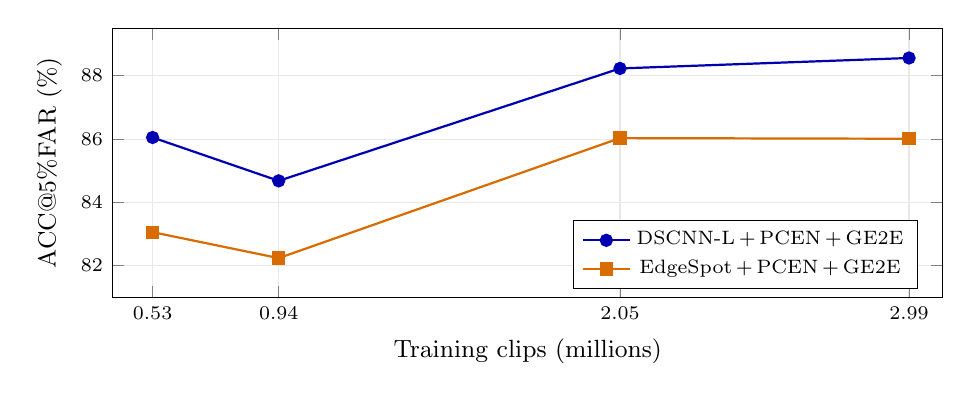
\begin{tikzpicture}
\begin{axis}[
  width=\columnwidth, height=5.0cm,
  xlabel={Training clips (millions)},
  ylabel={ACC@5\%FAR (\%)},
  xmin=0.4,xmax=3.1, ymin=81,ymax=89.5,
  xtick={0.53,0.94,2.05,2.99},
  xticklabels={0.53,0.94,2.05,2.99},
  legend pos=south east, legend style={font=\scriptsize},
  grid=both, grid style={gray!18},
  tick label style={font=\scriptsize},
  label style={font=\small},
]
\addplot[mark=*,thick,blue!70!black] coordinates
  {(0.53,86.05)(0.94,84.68)(2.05,88.23)(2.99,88.56)};
\addplot[mark=square*,thick,orange!85!black] coordinates
  {(0.53,83.06)(0.94,82.24)(2.05,86.03)(2.99,86.01)};
\legend{DSCNN-L\,+\,PCEN\,+\,GE2E, EdgeSpot\,+\,PCEN\,+\,GE2E}
\end{axis}
\end{tikzpicture}
\caption{Cross-corpus accuracy on GSC test100 versus training-data volume
(per-word caps $20/50/220/620$). Performance saturates near $\sim$2\,M clips.}
\label{fig:scale}
\end{figure}

\begin{table}[t]
\centering
\caption{Data-scale sweep (PCEN$+$GE2E), GSC test100. ACC at $5\%$ FAR.}
\label{tab:scale}
\footnotesize
\setlength{\tabcolsep}{3.5pt}
\begin{tabular}{l c r r r r}
\toprule
\textbf{Encoder} & \textbf{Cap} & \acc$_{5\%}$ & \auc & \eer & F1\\
\midrule
\multirow{4}{*}{DSCNN-L}
 & 20  & 86.05 & 91.57 & 16.25 & 75.90 \\
 & 50  & 84.68 & 90.45 & 17.42 & 74.34 \\
 & 220 & 88.23 & 93.87 & 12.78 & 80.67 \\
 & 620 & \best{88.56} & \best{94.04} & \best{12.53} & \best{81.02} \\
\midrule
\multirow{4}{*}{EdgeSpot}
 & 20  & 83.06 & 87.22 & 20.40 & 70.46 \\
 & 50  & 82.24 & 87.74 & 20.19 & 70.73 \\
 & 220 & \best{86.03} & 91.31 & 16.47 & 75.61 \\
 & 620 & 86.01 & \best{91.34} & 16.64 & 75.38 \\
\bottomrule
\end{tabular}
\end{table}

\paragraph{The SCAF collapse at $37$k classes.}
The most striking result of the scale study is a \emph{qualitative} failure.
On the $31$-class micro-set and the $\sim$500-class Top-500 split, SCAF and
SCAF$+$GE2E are excellent (AUC $\approx95$; see \Cref{sec:best}). However, on the
full $37{,}387$-class vocabulary with the default SCAF weight of $1.0$, training
\emph{collapses from epoch $2$}: validation AUC pins at $0.5000$, the GE2E
in-episode accuracy falls to $\approx0.033$ ($\approx1/30$, i.e.\ chance), and
the resulting GSC metrics are degenerate (AUC $50$, F1 $0$, $\frr{=}100\%$,
keyword ACC $9.09\%$). The mechanism is a gradient-magnitude imbalance: the
sub-center ArcFace logit scale ($s{=}30$) multiplied across $\sim$$3.7\times10^4$
classes produces a classification gradient that dwarfs the centroid/cosine
terms, driving all embeddings to a trivial solution. The same hybrid does
\emph{not} collapse under KD because there the SCAF weight is
$5\times10^{-5}$. The practical remedies we verify are: (i) reduce the SCAF
weight to $\sim$$5\times10^{-5}$, (ii) warm up the margin/scale, or (iii) drop
the classification term entirely and use GE2E or KD. This is a cautionary
result: \emph{angular-margin classification losses that are state-of-the-art at
$10^2$--$10^3$ classes do not transfer naively to $10^4$-class word embedding}.

\subsection{Q3: Knowledge distillation trades teacher knowledge for data}
\label{sec:kd}

We distill a frozen Wav2Vec\,2.0 teacher into the compact EdgeSpot student via the
cosine objective of \Cref{eq:kd} (loss \code{kd\_scaf}). \Cref{tab:kd} shows
that at cap-50 KD improves every metric over GE2E ($+3.60$ ACC@1\%FAR,
$-4.78$ EER, $+6.31$ F1) and, strikingly, \emph{KD at cap-50 matches GE2E at
cap-220} --- the same accuracy with roughly half the training clips. KD also
saturates early (cap-50 $\to$ cap-220 is essentially flat), indicating that the
teacher injects most of its useful inductive bias from limited data.

\begin{table}[t]
\centering
\caption{Knowledge distillation vs.\ GE2E (EdgeSpot student), GSC test100.
KD at cap-50 matches GE2E at cap-220.}
\label{tab:kd}
\footnotesize
\setlength{\tabcolsep}{3.5pt}
\begin{tabular}{l l r r r r}
\toprule
\textbf{Cap} & \textbf{Loss} & \acc$_{1\%}$ & \acc$_{5\%}$ & \eer & F1\\
\midrule
50  & GE2E       & 77.14 & 82.24 & 20.19 & 70.73 \\
\rowcolor{blue!7}
50  & KD         & \best{80.74} & \best{85.82} & \best{15.41} & \best{77.04} \\
220 & GE2E       & {--} & 86.03 & 16.47 & 75.61 \\
220 & KD         & 80.82 & 85.90 & 15.36 & 77.10 \\
\bottomrule
\end{tabular}
\end{table}

\subsection{Q4: Best deployable systems}
\label{sec:best}

\Cref{tab:final} consolidates the strongest configurations per data regime.
Three operating points are worth highlighting:

\begin{itemize}[leftmargin=1.2em,itemsep=2pt]
\item \textbf{Best overall accuracy}: DSCNN-L\,+\,PCEN\,+\,GE2E (cap-620,
composite epoch selection) reaches \best{$86.36\pm1.29$} open-set ACC@1\%FAR and
$89.93\pm0.65$ at $5\%$ FAR, with AUC $95.21$, EER $11.32$, F1 $82.73$, keyword
ACC $92.92\%$.
\item \textbf{Best compact}: EdgeSpot-Full\,+\,PCEN\,+\,GE2E (cap-620) reaches
$82.87\pm1.22$ ACC@1\%FAR at $0.131$\,M parameters --- within $\sim$3.5 points of
the best system at one third the size, and competitive with the EdgeSpot-4
literature reference ($\sim$82\% ACC@1\%FAR, $\sim$128k params).
\item \textbf{Best small-vocabulary}: on the reduced Top-500 split, the
EdgeSpot\,+\,PCEN\,+\,SCAF$+$GE2E hybrid is the strongest compact model
($85.62\pm1.04$ ACC@1\%FAR, AUC $95.34$), confirming that the hybrid is excellent
\emph{when the class count is small enough not to trigger the collapse}.
\end{itemize}

\begin{table*}[t]
\centering
\caption{Consolidated best systems across data regimes (GSC \textbf{test100},
EdgeSpot-exact $10$-shot, $100$ runs). ACC and FRR at the stated FAR; lower is
better for EER/FRR, higher for the rest. ``coll.''\ = degenerate collapse.}
\label{tab:final}
\small
\setlength{\tabcolsep}{4.5pt}
\begin{tabular}{l l l c r r r r r r}
\toprule
\textbf{Regime (\#words)} & \textbf{Encoder} & \textbf{Loss} & \textbf{Params} &
\acc$_{1\%}$ & \acc$_{5\%}$ & \auc & \eer & F1 & KW-ACC\\
\midrule
Micro-set ($31$)   & EdgeSpot & SCAF+GE2E (locked) & 0.131\,M & 84.61 & 86.12 & 95.61 & 11.54 & 82.41 & 77.66 \\
Top-500 ($500$)    & EdgeSpot & SCAF+GE2E (ep13)   & 0.131\,M & 85.62 & 88.79 & 95.34 & 11.51 & 82.45 & 90.44 \\
Top-500 ($500$)    & DSCNN-L  & GE2E               & 0.413\,M & 81.55 & 86.56 & 93.17 & 14.00 & 78.97 & 88.62 \\
Full cap-20 ($37$k)  & DSCNN-L & GE2E              & 0.413\,M & 82.10 & 86.05 & 91.57 & 16.25 & 75.90 & 88.90 \\
Full cap-220 ($37$k) & DSCNN-L & GE2E              & 0.413\,M & {--}  & 88.23 & 93.87 & 12.78 & 80.67 & 89.82 \\
\rowcolor{blue!7}
Full cap-620 ($37$k) & DSCNN-L & GE2E (ep300)      & 0.413\,M & \best{86.36} & \best{89.93} & \best{95.21} & \best{11.32} & \best{82.73} & \best{92.92} \\
Full cap-620 ($37$k) & EdgeSpot & GE2E (ep300)     & 0.131\,M & 82.87 & 86.76 & 92.41 & 14.82 & 77.85 & 87.29 \\
Full cap-50 ($37$k)  & EdgeSpot & KD               & 0.131\,M & 80.74 & 85.82 & 91.19 & 15.41 & 77.04 & 87.95 \\
Full cap-220 ($37$k) & EdgeSpot & SCAF+GE2E ($w{=}1$) & 0.131\,M & {coll.} & {coll.} & 50.00 & 50.00 & {coll.} & 9.09 \\
\bottomrule
\end{tabular}
\end{table*}

\paragraph{Reproducibility note on data regimes.}
Within the full-vocabulary results, three cap-620 runs use different episode
budgets (a $40$-epoch fixed screen, a long $1000$-episode saturation run, and a
$300$-episode composite-selection development run). They must not be conflated;
\Cref{tab:matrix,tab:scale,tab:final} draw each row from a single consistent run,
and the table captions state the budget where it matters.

%==============================================================================
\section{System Implementation}\label{sec:system-impl}

Beyond the core encoder, the project ships a complete, dependency-light
deployment stack. Audio I/O uses \code{soundfile}/\code{scipy} (no torchaudio
runtime dependency) to remain compatible with a CUDA-10.2 server.

\paragraph{Denoising (EXT-1).}
A unified \code{Denoiser} exposes two backends: a CPU-friendly spectral-gating
denoiser (\code{noisereduce}, with an RMS-guard fallback that prevents
over-suppression of short keyword clips) and an optional neural enhancer
(SpeechBrain MetricGAN+). Denoising is a runtime toggle and never blocks the
core pipeline.

\paragraph{Streaming and VAD (EXT-2).}
A CPU streaming engine performs sliding-window detection ($1$\,s window,
$0.5$\,s stride) gated by Silero VAD: only windows that VAD marks as speech are
embedded and matched, reducing computation and false activations on silence.
A backend-agnostic \emph{state machine} (\Cref{alg:sm}) stabilizes raw
candidates into clean events using majority-vote smoothing over a short window,
a top-2 margin check, and a cooldown to suppress duplicate firings.

\begin{algorithm}[t]
\caption{Streaming decision state machine (smoothing $+$ cooldown).}
\label{alg:sm}
\footnotesize
\begin{algorithmic}[1]
\Require window $W$, votes $V$, margin $m_{\min}$, cooldown $C$
\State buffer $\gets$ deque(maxlen $=W$); \ $t_{\text{last}}\gets-\infty$
\For{each candidate $c$ with $[t_s,t_e]$}
  \If{$t_s - t_{\text{last}} < C$} \State emit \textsc{cooldown}; \textbf{continue} \EndIf
  \If{$\lnot c.\text{detected}$ \textbf{or} $c.\text{kw}{=}$\texttt{unknown}
       \textbf{or} $c.\text{margin}<m_{\min}$}
       \State clear buffer; emit \textsc{rejected}; \textbf{continue}
  \EndIf
  \State push $c$; \ $k^\star\gets$ majority keyword in buffer
  \If{votes$(k^\star)\ge V$}
     \State $a\gets\arg\max_{\text{conf}}\{c\in\text{buffer}:c.\text{kw}{=}k^\star\}$
     \State $t_{\text{last}}\gets a.t_e$; clear buffer; emit \textsc{detected}$(k^\star)$
  \Else\ \State emit \textsc{scoring} \EndIf
\EndFor
\end{algorithmic}
\end{algorithm}

\paragraph{Optional speaker gate.}
An ECAPA-TDNN speaker-verification gate (enroll-then-verify by cosine
similarity) can restrict detections to an enrolled speaker; like denoising it is
optional and fail-open.

\paragraph{Web demonstrator.}
A FastAPI backend and a React front-end provide an offline demo with
hot-swappable checkpoints (auto-discovery, path loading, and direct file
upload), long-audio timing analysis, and a sampled $17$-known/$17$-unknown
open-set evaluation. We stress that the in-UI sampled evaluation is a
calibration/illustration tool and does \emph{not} replace the EdgeSpot-exact
test-set protocol used for all reported numbers.

\paragraph{Latency budget.}
The streaming pipeline is designed to a per-component CPU budget (VAD
$<5$\,ms/chunk, MFCC $<5$\,ms, encoder $<10$\,ms, classifier $<1$\,ms; core
$<21$\,ms; $<51$\,ms with denoising; $<71$\,ms with speaker verification;
$<100$\,ms end-to-end). These are design targets; a measured field benchmark
(false-alarms/hour, miss rate, wall-clock latency on target hardware) is left to
future work.

%==============================================================================
\section{Discussion}\label{sec:discuss}

\paragraph{Why GE2E and PCEN win.}
GE2E optimizes the \emph{same} enroll-then-match objective used at deployment
(\Cref{eq:proto,eq:score}), so the train/test objective gap is minimal; triplet
optimizes a proxy (relative pairwise margins) and classification losses optimize
a closed-set decision boundary that is discarded at test time. PCEN's
per-channel adaptive compression normalizes the large dynamic range of
cross-corpus recordings (MSWC$\to$GSC), which matters more for the smaller edge
encoder (largest PCEN gain), consistent with the front-end carrying relatively
more of the representational burden when the backbone is small.

\paragraph{Why classification collapses at scale.}
The collapse is not a tuning artifact but a structural mismatch: angular-margin
softmax couples \emph{all} classes through a single normalized weight matrix, so
its gradient norm grows with class count, while GE2E/cosine-KD gradients are
bounded per episode/sample. At $37$k classes the classification term overwhelms
the metric terms unless down-weighted by $\sim$$10^{-4}$ or removed. This
generalizes a known practical lesson from face recognition (where careful
scale/margin scheduling is essential at large identity counts) to large-vocabulary
word embedding.

\paragraph{Capacity vs.\ data.}
DSCNN-L ($3.2\times$ larger) consistently leads on accuracy, but the gap to the
compact EdgeSpot ($\sim$3.5 ACC points) is small relative to the size saving, and
KD narrows the data requirement of the compact model. For tight edge budgets,
EdgeSpot\,+\,PCEN\,+\,GE2E (optionally KD-initialized) is the recommended
operating point; for best accuracy, DSCNN-L\,+\,PCEN\,+\,GE2E.

%==============================================================================
\section{Limitations}\label{sec:limits}

(i) ACC@FAR/FRR@FAR use ROC-derived (oracle) thresholds rather than thresholds
transferred from an independent calibration split; we mitigate this by always
co-reporting threshold-free AUC/EER/F1. (ii) Enrollment is fixed at $k{=}10$
shots throughout; a $k$-shot sensitivity sweep ($k{\in}\{1,3,5\}$) is not
included. (iii) The streaming/denoising latency figures are design budgets, not
measured field benchmarks, and there is no quantitative denoising ablation
(SNR-sweep accuracy). (iv) Some large-vocabulary runs were epoch-limited by
cloud-session constraints; the Top-500 epoch-25 point is reported from training
logs rather than a locked artifact and is excluded from headline claims.

%==============================================================================
\section{Conclusion}\label{sec:conclusion}

We presented a controlled study of few-shot open-set keyword spotting trained at
true vocabulary scale (up to $37{,}387$ words) and evaluated cross-corpus under a
strict $10$-shot, $100$-run protocol. The trainable PCEN front-end and the
centroid GE2E objective are the two robust, transferable wins; a frozen-teacher
cosine distillation halves the data needed by the compact encoder; and, most
importantly, we documented and explained a catastrophic collapse of sub-center
ArcFace at $10^4$-class scale, with a simple weighting fix. The best system
(DSCNN-L\,+\,PCEN\,+\,GE2E) attains $86.36\%$ open-set accuracy at $1\%$ FAR and
$95.21$ AUC on GSC, while a $3.2\times$ smaller edge model stays within a few
points. We release code, protocols, and an offline demonstrator to support
reproduction. Future work includes a $k$-shot sensitivity study, a measured
on-device latency/false-alarm benchmark, an SNR-sweep denoising ablation, and
warm-up/curriculum schedules to stabilize angular-margin losses at scale.

%==============================================================================
\section*{Reproducibility}
All experiments use fixed seeds (seed $42$, cuDNN determinism). Training,
evaluation, and the EdgeSpot-exact protocol are scripted
(\code{scripts/train.py}, \code{scripts/evaluate.py},
\code{scripts/evaluate\_edgespot\_protocol.py}); per-run JSON artifacts store the
seed, positive/negative word partition, and all metrics for each of the $100$
runs. The web demonstrator runs fully offline.

%==============================================================================
\begin{thebibliography}{99}
\footnotesize

\bibitem{zhang2017hello}
Y.~Zhang, N.~Suda, L.~Lai, and V.~Chandra,
``Hello edge: Keyword spotting on microcontrollers,''
\emph{arXiv:1711.07128}, 2017.

\bibitem{kim2021bcresnet}
B.~Kim, S.~Chang, J.~Lee, and D.~Sung,
``Broadcasted residual learning for efficient keyword spotting,''
\emph{Interspeech}, 2021.

\bibitem{snell2017prototypical}
J.~Snell, K.~Swersky, and R.~Zemel,
``Prototypical networks for few-shot learning,''
\emph{NeurIPS}, 2017.

\bibitem{schroff2015facenet}
F.~Schroff, D.~Kalenichenko, and J.~Philbin,
``FaceNet: A unified embedding for face recognition and clustering,''
\emph{CVPR}, 2015.

\bibitem{wan2018ge2e}
L.~Wan, Q.~Wang, A.~Papir, and I.~L.~Moreno,
``Generalized end-to-end loss for speaker verification,''
\emph{ICASSP}, 2018.

\bibitem{deng2019arcface}
J.~Deng, J.~Guo, N.~Xue, and S.~Zafeiriou,
``ArcFace: Additive angular margin loss for deep face recognition,''
\emph{CVPR}, 2019.

\bibitem{deng2020subcenter}
J.~Deng, J.~Guo, T.~Liu, M.~Gong, and S.~Zafeiriou,
``Sub-center ArcFace: Boosting face recognition by large-scale noisy web faces,''
\emph{ECCV}, 2020.

\bibitem{bendale2016openmax}
A.~Bendale and T.~E.~Boult,
``Towards open set deep networks,''
\emph{CVPR}, 2016.

\bibitem{liu2020energy}
W.~Liu, X.~Wang, J.~Owens, and Y.~Li,
``Energy-based out-of-distribution detection,''
\emph{NeurIPS}, 2020.

\bibitem{wang2017trainable}
Y.~Wang, P.~Getreuer, T.~Hughes, R.~F.~Lyon, and R.~A.~Saurous,
``Trainable frontend for robust and far-field keyword spotting,''
\emph{ICASSP}, 2017.

\bibitem{baevski2020wav2vec}
A.~Baevski, H.~Zhou, A.~Mohamed, and M.~Auli,
``wav2vec 2.0: A framework for self-supervised learning of speech
representations,'' \emph{NeurIPS}, 2020.

\bibitem{mazumder2021mswc}
M.~Mazumder \emph{et al.},
``Multilingual Spoken Words Corpus,''
\emph{NeurIPS Datasets and Benchmarks}, 2021.

\bibitem{warden2018speech}
P.~Warden,
``Speech Commands: A dataset for limited-vocabulary speech recognition,''
\emph{arXiv:1804.03209}, 2018.

\end{thebibliography}

\end{document}
